\subsection{Metriche software}
\subsubsection{Versioni del browser supportate}
\begin{figure}[h]
	\centering
	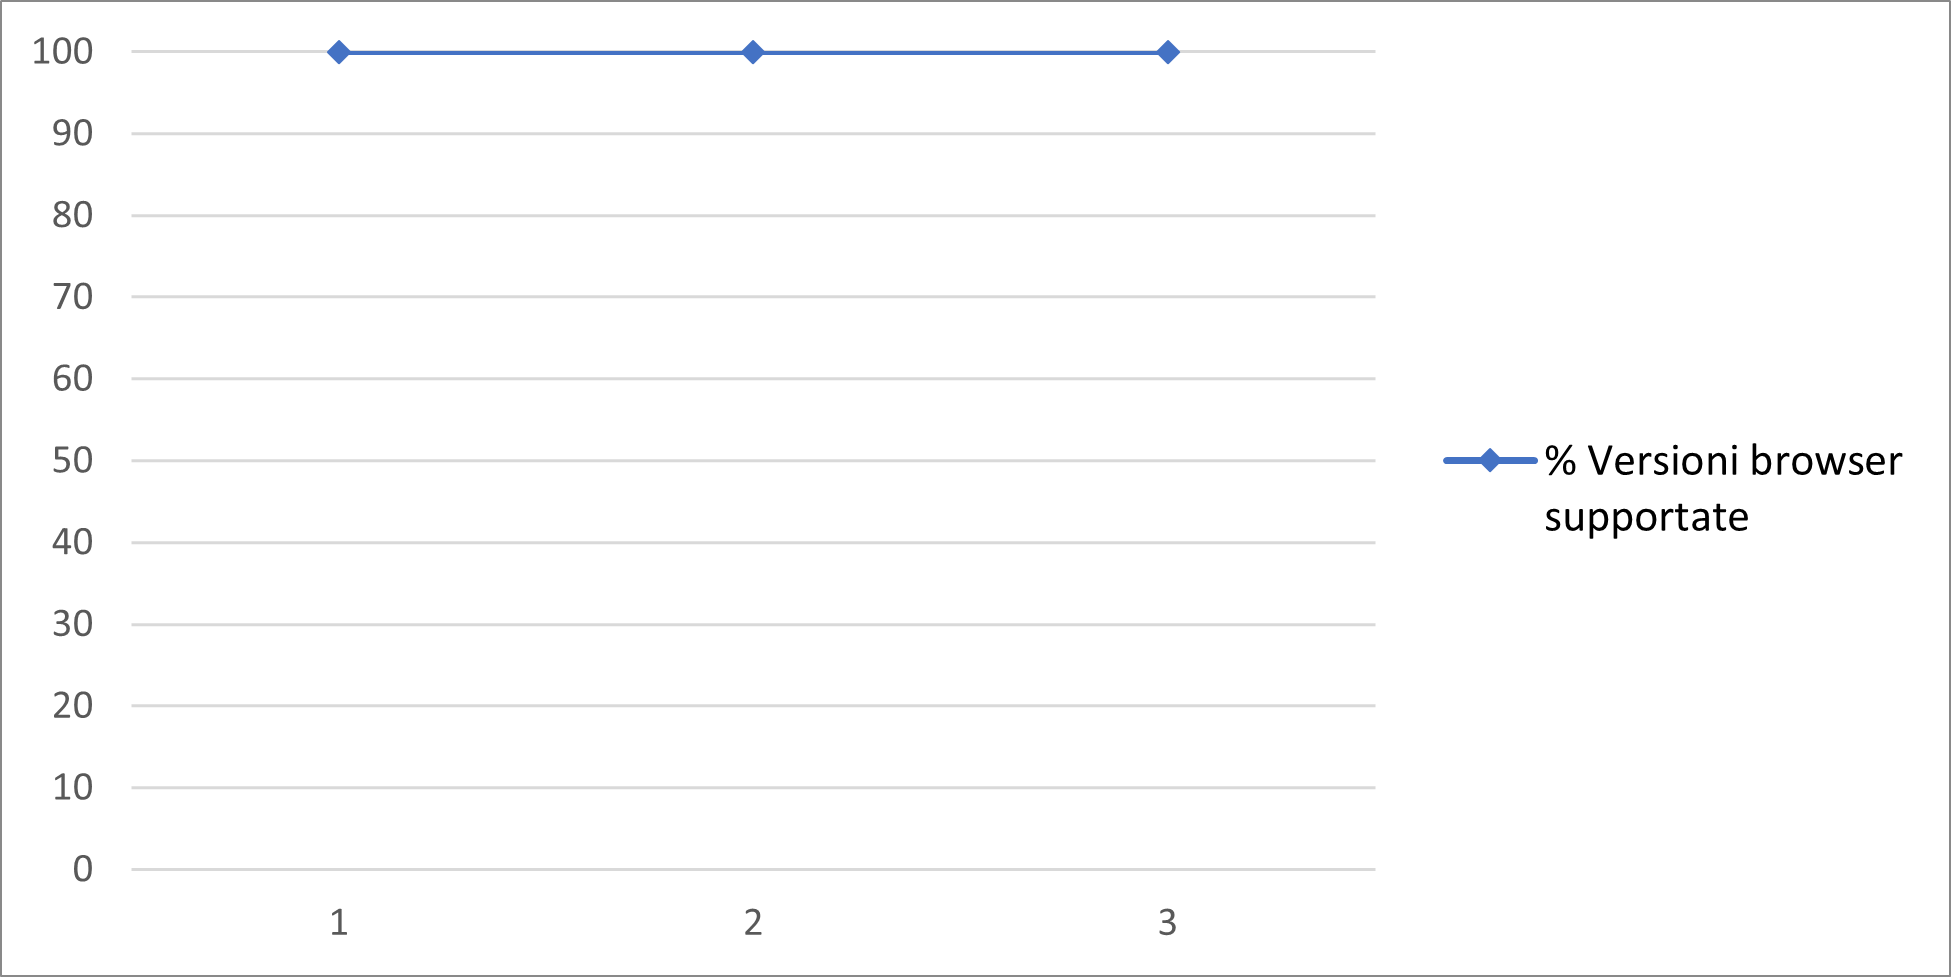
\includegraphics[width=13cm]{Images/BrowserSupportati.png}
	\caption{Grafico delle versioni browser supportate nel periodo di progettazione della technology baseline.}
\end{figure}

\subsubsection{Copertura dei requisiti}
\begin{figure}[h]
	\centering
	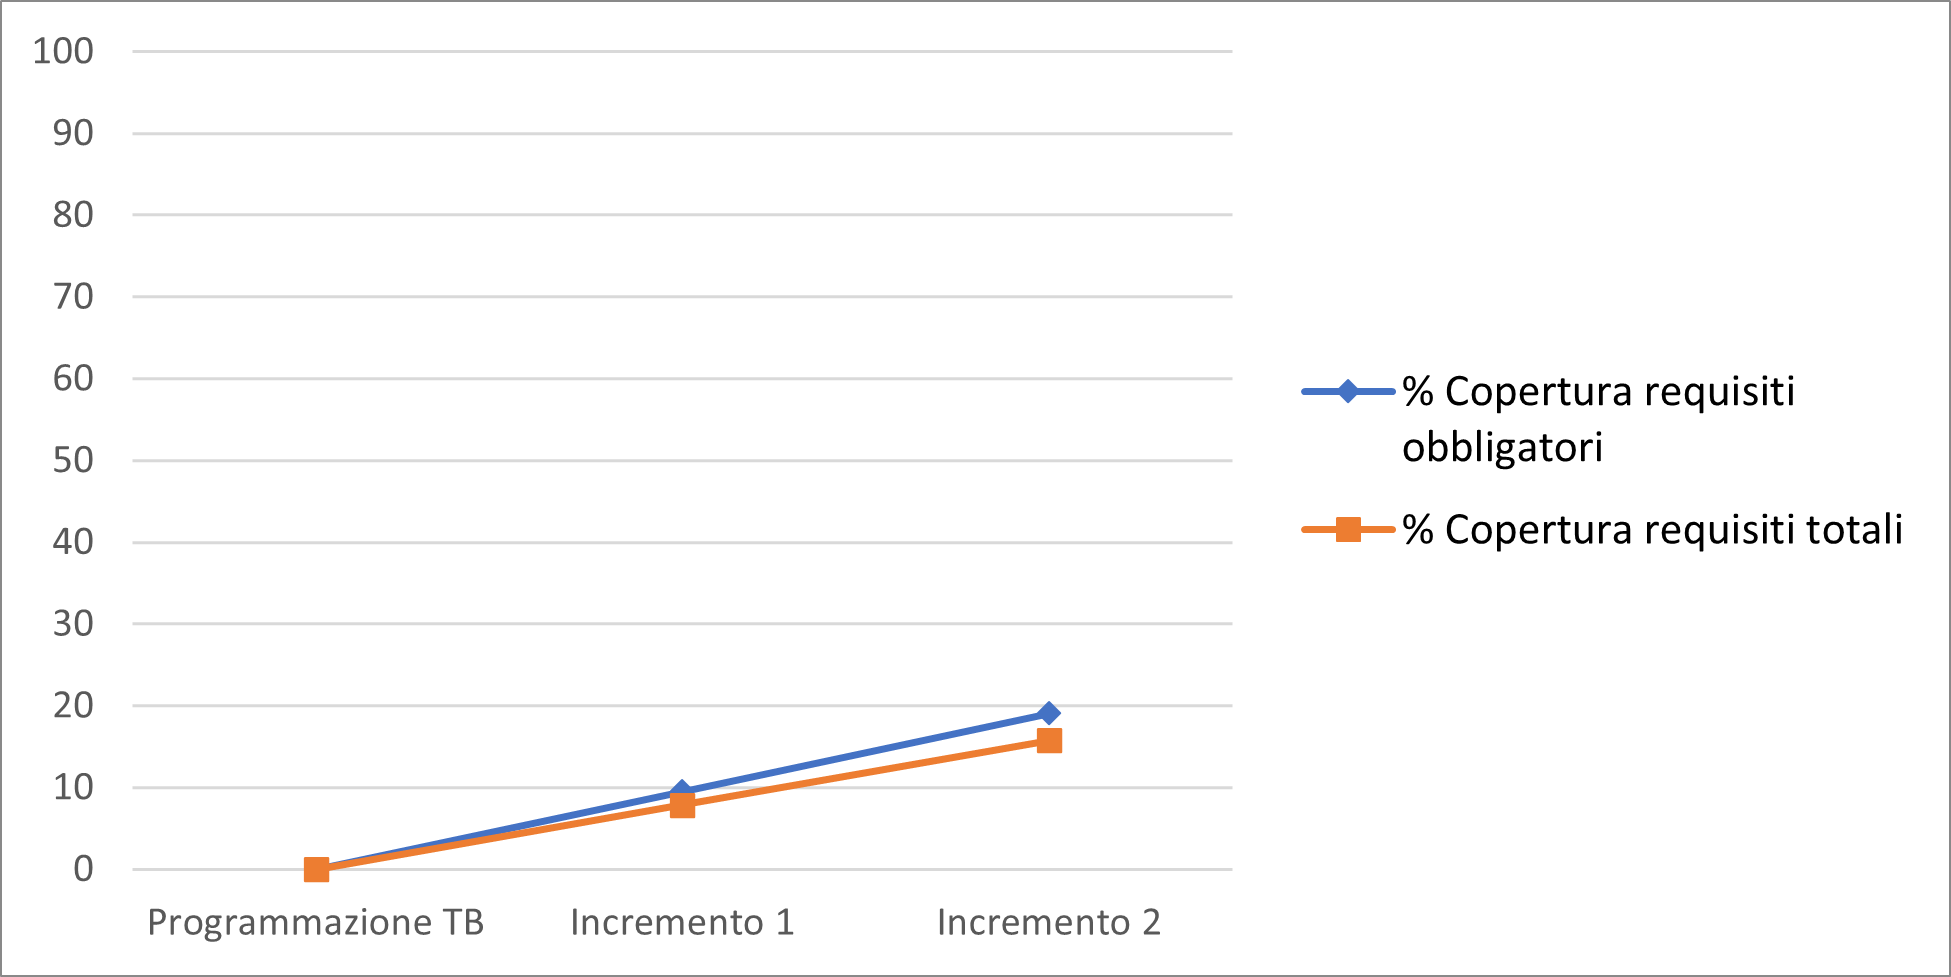
\includegraphics[width=14cm]{Images/CoperturaRequisiti.png}
	\caption{Grafico del numero di requisiti soddisfatti nel periodo di progettazione della technology baseline.}
\end{figure}

\newpage
\subsubsection{Average Cyclomatic complexity}
\begin{figure}[h]
	\centering
	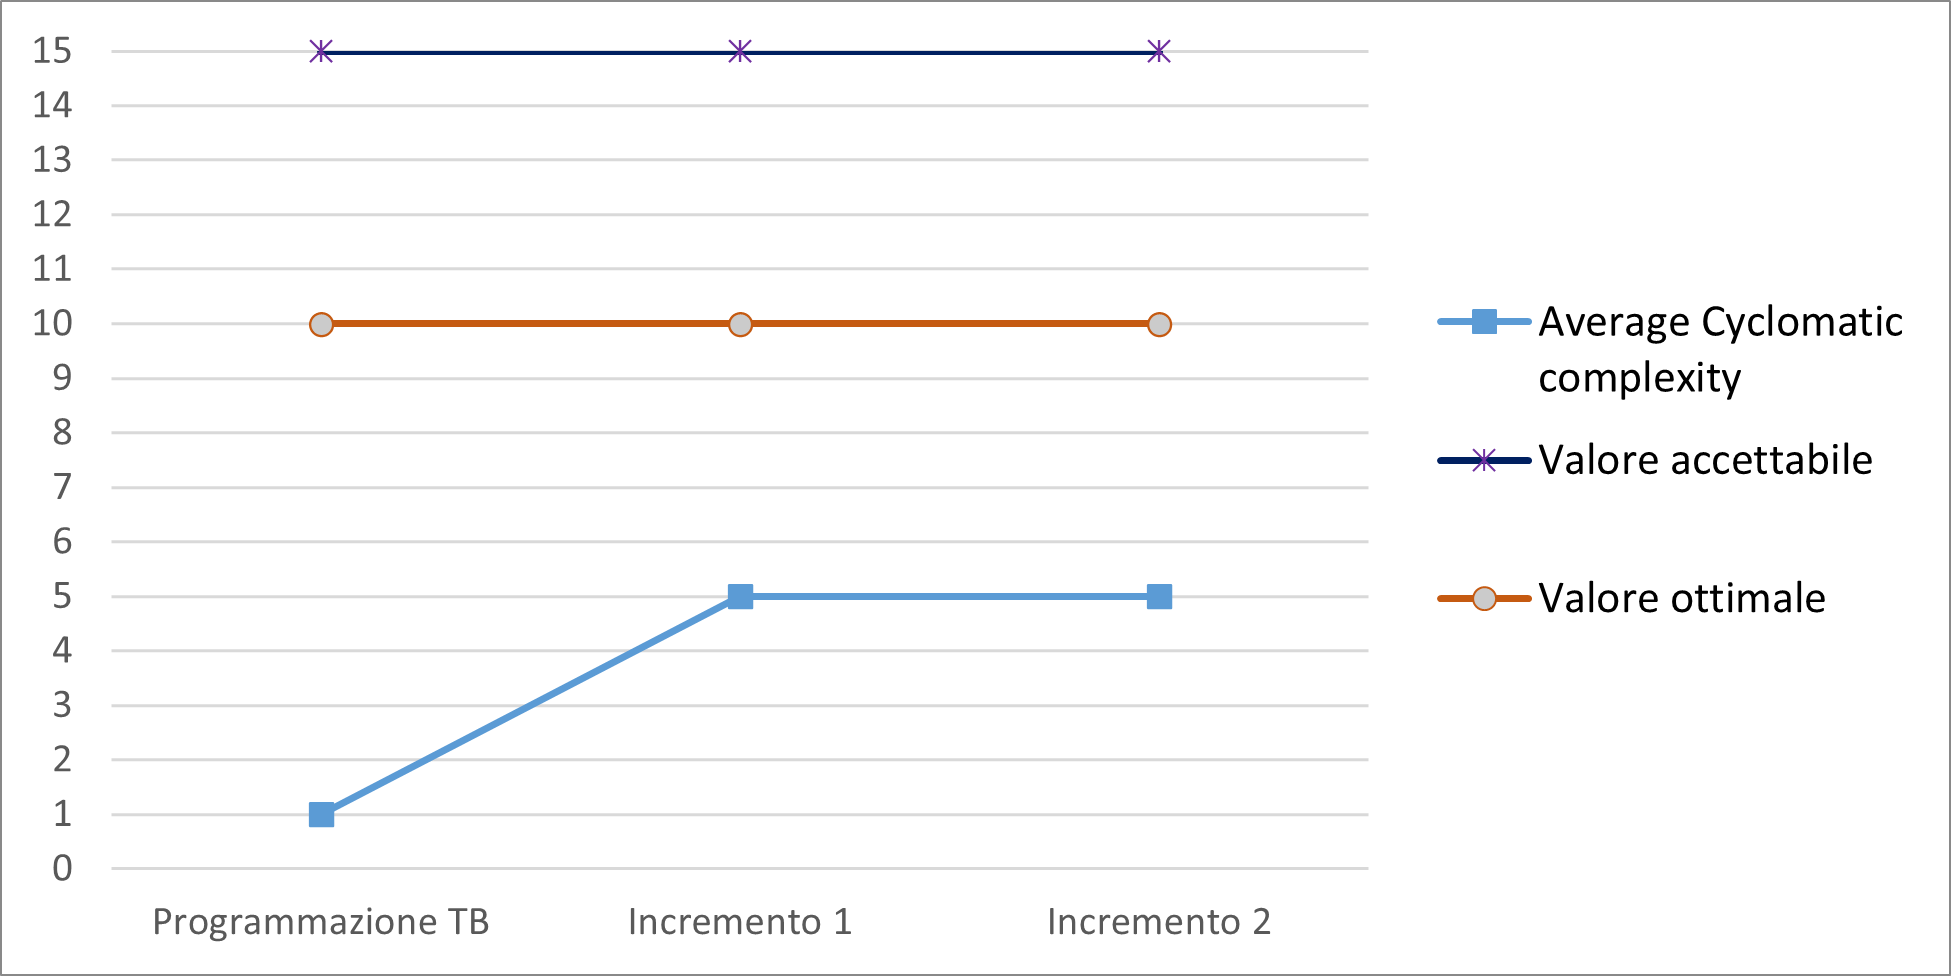
\includegraphics[width=14cm]{Images/CyclomaticComplexity.png}
	\caption{Grafico complessità ciclomatica nel periodo di progettazione della technology baseline.}
\end{figure}

% \subsubsection{Comprensione del codice} DA TOGLIERE?

\subsubsection{Tempo medio di risposta}
\begin{figure}[h]
	\centering
	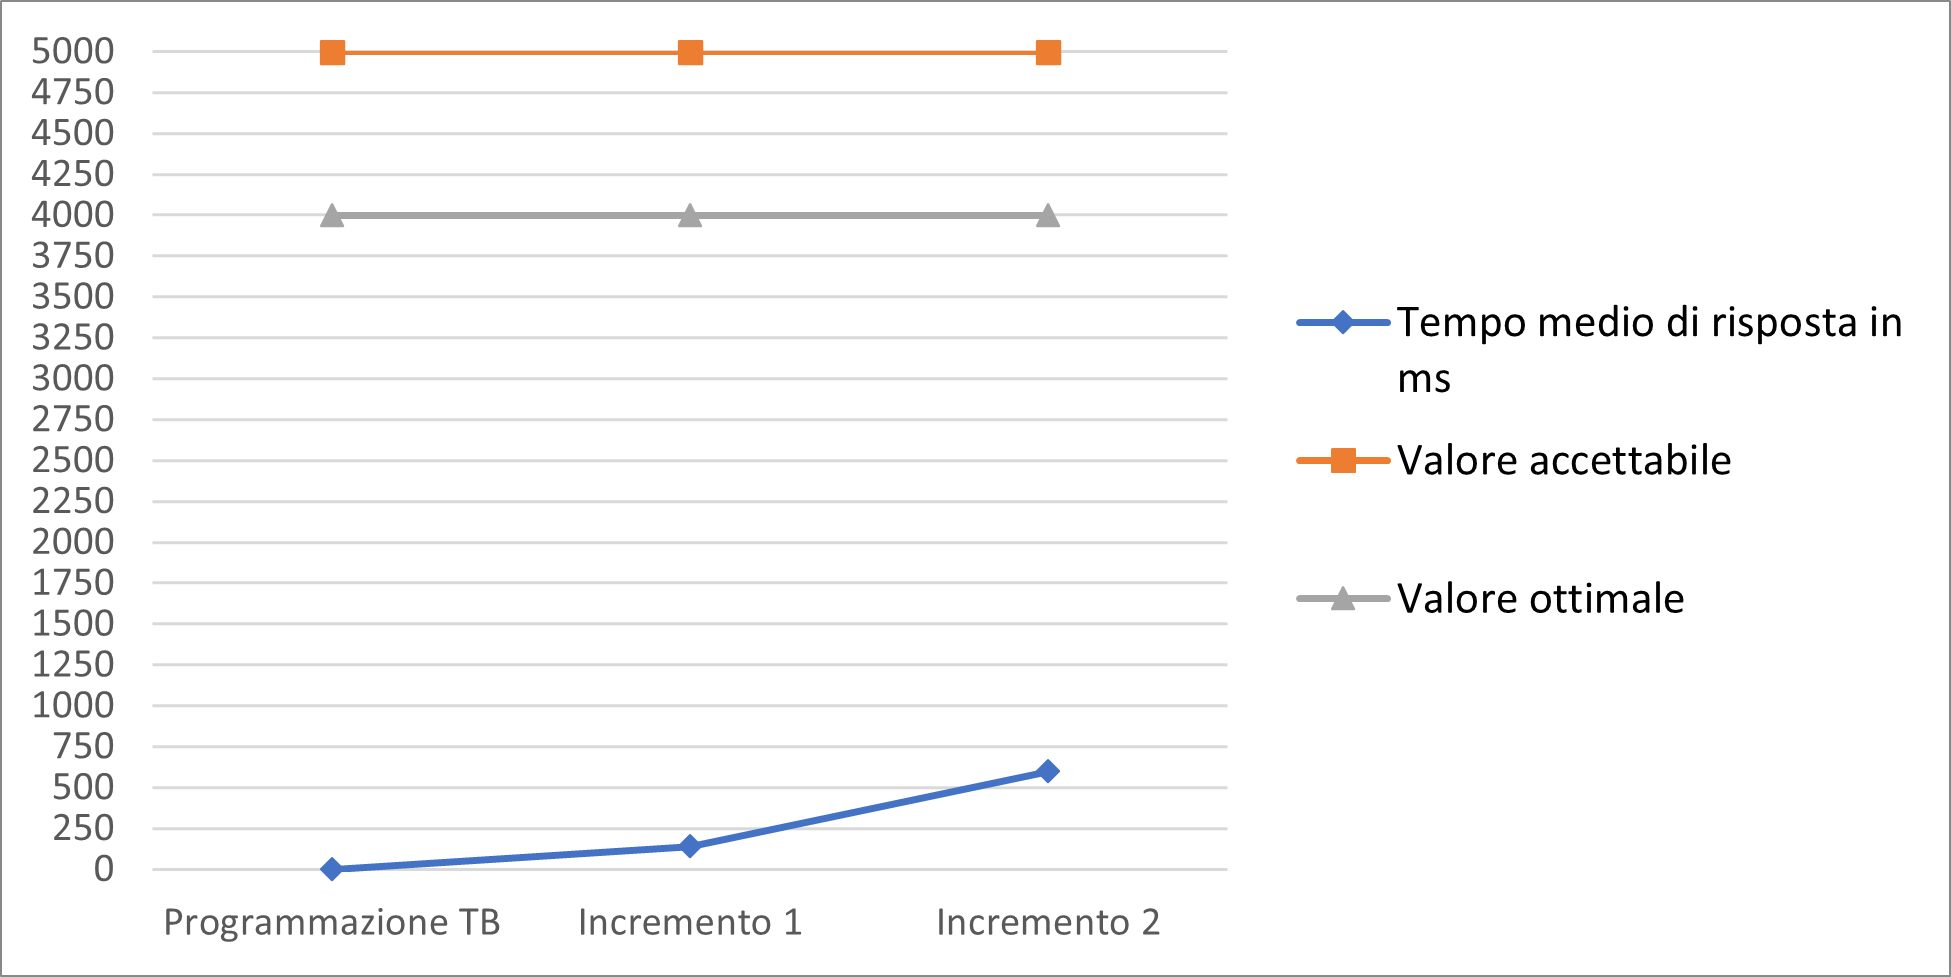
\includegraphics[width=14cm]{Images/TempoMedioRisposta.png}
	\caption{Grafico risposta media nel periodo di progettazione della technology baseline.}
\end{figure}

\newpage
\subsubsection{Facilità di utilizzo}
\begin{figure}[h]
	\centering
	\includegraphics[width=14cm]{Images/FacilitàUtilizzo.png}
	\caption{Grafico della facilità di utilizzo nel periodo di progettazione della technology baseline.}
\end{figure}

\subsubsection{Facilità apprendimento funzionalità}
\begin{figure}[h]
	\centering
	\includegraphics[width=14cm]{Images/FacilitàApprendimento.png}
	\caption{Grafico della facilità di apprendimento nel periodo di progettazione della technology baseline.}
\end{figure}

\newpage
\subsubsection{Densità di failure}
\begin{figure}[h]
	\centering
	\includegraphics[width=14cm]{Images/DensitàFailure.png}
	\caption{Grafico desità di failure media nel periodo di progettazione della technology baseline.}
\end{figure}